\documentclass[10pt]{article}
\usepackage{amsmath}
\usepackage{geometry}
\usepackage{fancybox}
\usepackage{tikz}
\usepackage{listings}
 \geometry{
 a4paper,
 total={170mm,257mm},
 left=20mm,
 top=10mm,
 bottom=15mm
 }
 
\usepackage{color}
 
\definecolor{codegreen}{rgb}{0,0.6,0}
\definecolor{codegray}{rgb}{0.5,0.5,0.5}
\definecolor{codepurple}{rgb}{0.58,0,0.82}
\definecolor{backcolour}{rgb}{0.95,0.95,0.92}

\linespread{1.3}

\title{CSC263H1 Assignment 3}
\author{Jiatao Xiang, Xu Wang, Huakun Shen}
\date{February 14th, 2019}

\begin{document}
\maketitle

\lstdefinestyle{mystyle}{
    backgroundcolor=\color{backcolour},   
    commentstyle=\color{codegreen},
    keywordstyle=\color{magenta},
    numberstyle=\tiny\color{codegray},
    stringstyle=\color{codepurple},
    basicstyle=\footnotesize,
    breakatwhitespace=false,         
    breaklines=true,                 
    captionpos=b,                    
    keepspaces=true,                 
    numbers=left,                    
    numbersep=5pt,                  
    showspaces=false,                
    showstringspaces=false,
    showtabs=false,                  
    tabsize=2
}
\lstset{style=mystyle}

\section*{Question 1}
\textbf{Insert:}\\
\ovalbox{
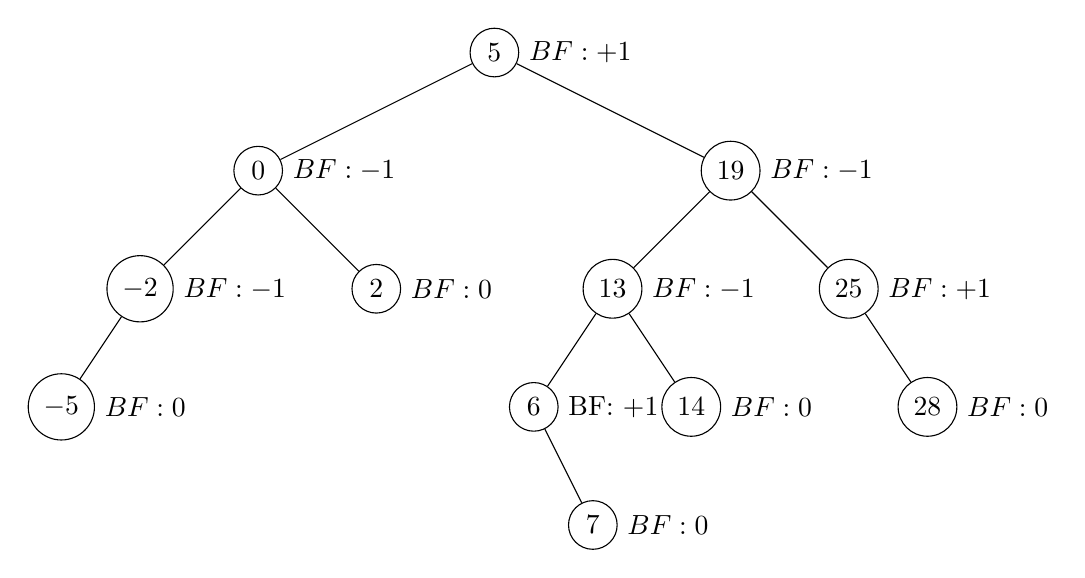
\begin{tikzpicture}[level/.style={sibling distance=60mm/#1}]
\node [circle,draw, label=right:$BF: +1$] (z){$5$}
  child {node [circle,draw, label=right:$BF: -1$] (lz) {$0$}
    child {node [circle,draw, label=right:$BF: -1$] (llz) {$-2$}
      child {node [circle, draw, label=right:$BF: 0$] (lllz) {$-5$}}
      child[fill=none]{edge from parent[draw=none]} 
    }
    child {node [circle,draw, label=right:$BF: 0$] (lrz) {$2$}
    }
  }
  child {node [circle,draw, label=right:$BF: -1$] (rz) {$19$}
    child {node [circle,draw, label=right:$BF: -1$] (rlz) {$13$}
    	child {node [circle, draw, label=right:BF: +1] (rllz) {$6$}
    		child[fill=none]{edge from parent[draw=none]}
    		child {node [circle, draw, label=right:$BF: 0$] (rllrz) {$7$}}
    	}
    	child {node [circle, draw, label=right:$BF: 0$] (rlrz) {$14$}}
    }
  child {node [circle,draw, label=right:$BF: +1$] (rrz) {$25$}
    child[fill=none]{edge from parent[draw=none]}
    child {node [circle, draw, label=right:$BF: 0$] (rrrz) {$28$}}		
	}
};
\end{tikzpicture}
}

\textbf{delete:}\\
\ovalbox{
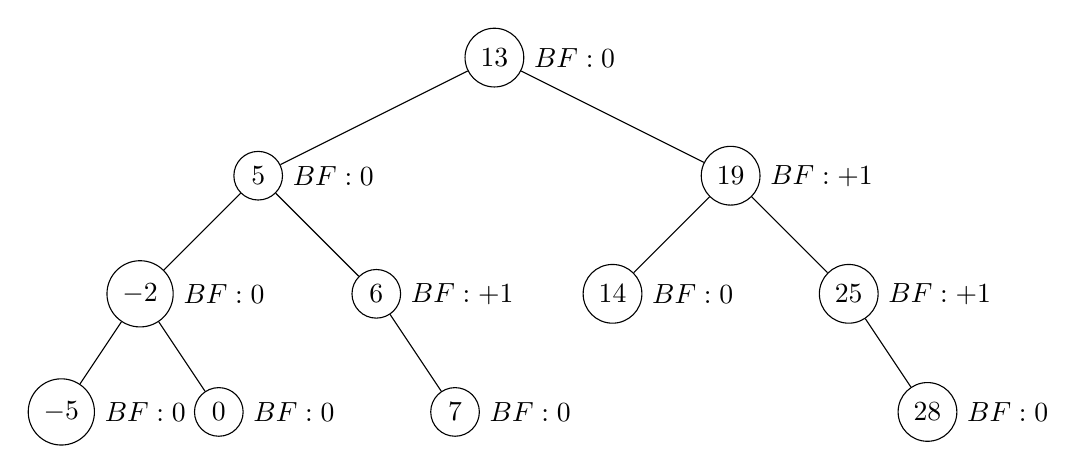
\begin{tikzpicture}[level/.style={sibling distance=60mm/#1}]
\node [circle,draw, label=right:$BF: 0$] (z){$13$}
  child {node [circle,draw, label=right:$BF: 0$] (lz) {$5$}
    child {node [circle,draw, label=right:$BF: 0$] (llz) {$-2$}
      child {node [circle, draw, label=right:$BF: 0$] (lllz) {$-5$}}
      child {node [circle, draw, label=right:$BF: 0$] (lllz) {$0$}}
    }
    child {node [circle,draw, label=right:$BF: +1$] (lrz) {$6$}
    	child[fill=none]{edge from parent[draw=none]}
    	child {node [circle, draw, label=right:$BF: 0$] (b) {$7$}}
    }
  }
  child {node [circle,draw, label=right:$BF: +1$] (rz) {$19$}
    child {node [circle,draw, label=right:$BF: 0$] (rlz) {$14$}
    }
  child {node [circle,draw, label=right:$BF: +1$] (rrz) {$25$}
    child[fill=none]{edge from parent[draw=none]}
    child {node [circle, draw, label=right:$BF: 0$] (rrrz) {$28$}}		
	}
};
\end{tikzpicture}
}
\section*{Question 2}
\begin{enumerate}
\item[a.]Description:\\
Define a new data structure, D, which is a AVL tree. Each of its node contains identifier, price and rating, and we set its identifier as key.\\
AddBook(D, x): we perform the insert operation(which also includes rebalancing) of an AVL tree that we discussed in lecture. One thing to be noticed is the key is identifier. This takes $\mathcal{O}(\log{}n)$\\
SearchBook(D, id): we perform the search operation of an AVL tree that we discussed in lecture. This takes $\mathcal{O}(\log{}n)$\\
\item[b.]
Description:\\
We add one more AVL tree such that each of its node contains price (which is also the key), the pointer to points its left child, the pointer points to its right child, and the max\_rating that stores the maximum rating among all nodes in the subtree rooted at the current node.\\
We use recursive algorithm to achieve the operation. The base case happens when D is leaf, thus, it has only two conditions to discuss. First Case: when D's price is less than or equal to input p, the max\_rating is the rating of D, thus, D.rating is returned. Second Case: when D's price is greater than input p, -1 is returned.\\
We start with the root of D, there exist three conditions.\\
First, when D has only right children: if $D.price \leq p$, we need to check the max\_rating of right subtree and D's rating, and return the greater one. If $D.price > p$, -1 is returned, because there is no node satisfies the requirement.\\Second, when D has only left children: if $D.price \leq p$, we need to check the max\_rating of left subtree and D's rating, and return the greater one. If $D.price > p$, we call recursively to help us find the max\_rating of D's left subtree.\\Third, when D has both left and right child, if $D.price > p$, we call recursively to find the max\_rating of the left subtree. Otherwise, we return the max of BestBookRating(D.left, p), BestBookRating(D.right, p), D.rating.\\
Simply speaking, the algorithm will traverse downwards from the root of the tree and it will either go down to left side or right side or return value, so the max path it will go through is less than or equal to the height of the tree.\\
\begin{equation*}
  T(n)=\begin{cases}
    c, &base case\\
    2T( \lfloor\frac{n}{2}\rfloor) + c, &if 
  \end{cases}
\end{equation*}
\begin{lstlisting}[language=Python]
def BestBookRating(D, p):
	if D is leaf:
		if D.price <= p:
			return D.rating
		return -1
	elif D only has right child:
		if D.price <= p:
			return max(BestBookRating(D.right, p), D.rating)
		return -1
	elif D only has left child:
		if D.price <= p:
			return max(D.left.max_rating, D.rating)
		return BestBookRating(D.left, p)
	elif D has both left and right child:
		if D.price > p:
			return BestBookRating(D.left, p)
		return max(BestBookRating(D.left, p), BestBookRating(D.right, p), D.rating)
\end{lstlisting}

\item[c.]
\item[d.]
\item[e.]

\end{enumerate}



\section*{Question 3}
\begin{enumerate}
\item[a.] Our data structure is based on \textbf{hash table}.\\
\textbf{Idea:} Put every element of set \textbf{B} into a hash table. Then hash every element of set \textbf{A} to a
slot in the hash table, and check whether the element of \textbf{A} is in this slot. If it is not in the slot, then it means that the element of set \textbf{A} is not in set \textbf{B}.\\
\textbf{Pseudo Code:}\\
Suppose \textbf{$\alpha$ = 10}, that is, each slot contains a linked list with size of at most approximately 10 elements.\\
Suppose we have a hash table \textbf{\textit{T}} with a size of $\frac{n}{\alpha}$.\\
Suppose we have a hashing function \textit{\textbf{h(x)}} that would return the index of one of the slots of \textbf{T} given \textbf{\textit{x}} as a input. Also assume \textbf{SUHA}.
\begin{lstlisting}[language=Python]
def h(x, num_slot):
	return x % num_slot
\end{lstlisting}
\begin{lstlisting}[language=Python]
for element in B:
		linked_list = T[h(element, len(T))]
		linked_list.append(element)
		
result = []
for element in A:
		linked_list = T[h(element, len(T))]
		for item in linked_list:
				if element == item:
						break
		result.append(element)
\end{lstlisting}
\item[b.]
Assumptions:\
\begin{itemize}
\item The linked list in each slot of hash table has approximately a length of $\alpha$ = 10
\item Hash table \textbf{T} has a length of $\frac{len(A)}{\alpha}$
\item SUHA for hash function \textbf{\textit{h(x, num\_slot)}}
\end{itemize}
Explanation:\
Part I: put \textbf{B} into \textbf{T}
\begin{enumerate}
\item[1.] Hashing function costs constant time
\item[2.] There are $n$ elements in \textbf{B}, performing hashing function \textbf{\textit{h}} for each element of \textbf{B} costs $\mathcal{O}(n\times1)$ of time.
\end{enumerate}
Part II: match element of \textbf{A} to \textbf{T}
\begin{enumerate}
\item[1.] Each linked list in each slot of \textbf{T} has a size of at most $\alpha$ (by \textbf{SUHA}), which is constant. In the worst case, we have to traverse through every linked list, which costs $\mathcal{O}(\alpha)=\mathcal{O}(1)$ of time.
\item[2.] There are $n$ elements in \textbf{A}, performing step 1 for each of them costs $\mathcal{O}(\alpha n)=\mathcal{O}(n)$ of time.
\end{enumerate}
Part I and Part II altogether cost $\mathcal{O}(n)$ of time.
\item[c.] In The worst case scenario, \textbf{SUHA} may not hold, and every element of B may be hashed into one single slot of \textbf{T}. Then when element of set \textbf{A} tries to find a matching element in this slot, it needs to traverse through the entire linked list and takes $\mathcal{O}(n)$ of time.\\
While there are $n$ elements in set \textbf{A}. If for each of the element in \textbf{A}, the program traverses through the linked list of size $n$ and do not exit early, it will take $\mathcal{O}(n\times n) = \mathcal{O}(n^2)$ of time.
\end{enumerate}


\end{document}
